\documentclass[11pt]{article}
\usepackage[T1]{fontenc}
\usepackage[utf8]{inputenc}
\usepackage{lmodern}
\usepackage{microtype}
\usepackage[margin=0.88in,headheight=15pt]{geometry}
\usepackage{amsmath,amssymb,amsthm,mathtools}
\usepackage{booktabs,longtable,array,tabularx}
\usepackage{enumitem}
\usepackage{xcolor}
\usepackage{listings}
\usepackage{tikz}
\usetikzlibrary{arrows.meta,positioning,fit,calc}
\usepackage{fancyhdr}
\usepackage{hyperref}
\usepackage{cleveref}
\usepackage{caption}
\usepackage{seqsplit}

\definecolor{navy}{HTML}{17324D}
\definecolor{teal}{HTML}{187F83}
\definecolor{bluegray}{HTML}{EAF0F4}
\definecolor{warmgray}{HTML}{F6F4F1}
\definecolor{codegray}{HTML}{4A5560}
\definecolor{accent}{HTML}{A44732}

\hypersetup{
  colorlinks=true,
  linkcolor=navy,
  citecolor=teal,
  urlcolor=teal,
  pdftitle={Contender 11: Self-Indexed Forest Reflection over Kind-Polymorphic System F-omega},
  pdfauthor={Prepared for the BusyLean project}
}

\pagestyle{fancy}
\fancyhf{}
\lhead{BusyLean Contender 11}
\rhead{Forest reflection over kind-polymorphic $F_\omega$}
\cfoot{\thepage}
\renewcommand{\headrulewidth}{0.35pt}

\lstdefinelanguage{lean}{
  keywords={def,theorem,inductive,structure,where,match,with,fun,let,in,
    namespace,end,open,abbrev,import,by,have,show,exact,obtain,refine,
    unfold,cases,rw,termination_by},
  sensitive=true,
  morecomment=[l]{--},
  morecomment=[s]{/-}{-/},
  morestring=[b]"
}
\lstset{
  language=lean,
  basicstyle=\ttfamily\footnotesize,
  keywordstyle=\bfseries\color{navy},
  commentstyle=\itshape\color{codegray},
  stringstyle=\color{accent},
  columns=fullflexible,
  keepspaces=true,
  showstringspaces=false,
  breaklines=true,
  frame=single,
  framerule=0.35pt,
  rulecolor=\color{navy!25},
  backgroundcolor=\color{warmgray},
  xleftmargin=0.6em,
  xrightmargin=0.6em,
  aboveskip=0.8em,
  belowskip=0.8em,
  literate=
    {→}{{$\to$}}1
    {←}{{$\leftarrow$}}1
    {≤}{{$\le$}}1
    {∈}{{$\in$}}1
    {∃}{{$\exists$}}1
    {∀}{{$\forall$}}1
    {⟨}{{$\langle$}}1
    {⟩}{{$\rangle$}}1
    {ω}{{$\omega$}}1
    {₁}{{$_1$}}1
    {₂}{{$_2$}}1
    {₃}{{$_3$}}1
}

\newtheorem{theorem}{Theorem}[section]
\newtheorem{lemma}[theorem]{Lemma}
\newtheorem{proposition}[theorem]{Proposition}
\theoremstyle{definition}
\newtheorem{definition}[theorem]{Definition}
\theoremstyle{remark}
\newtheorem{remark}[theorem]{Remark}

\newcommand{\N}{\mathbb{N}}
\newcommand{\Cten}{C_{10}}
\newcommand{\Celeven}{C_{11}}
\newcommand{\Fk}{\ensuremath{F_{\omega}^{\mathrm{kind}}}}
\newcommand{\lean}[1]{\texttt{#1}}
\newcommand{\snapshot}{\texttt{\seqsplit{4c4b03d0e2003c479e3bee90a21c8bea13f66c40}}}

\newenvironment{resultbox}{%
  \begin{center}\begin{minipage}{0.94\textwidth}
  \color{navy}\hrule height 1.2pt\vspace{0.65em}
}{%
  \vspace{0.65em}\hrule height 1.2pt
  \end{minipage}\end{center}
}

\title{\vspace{-1.2cm}\color{navy}\bfseries
  Contender 11: Self-Indexed Forest Reflection\\
  over Kind-Polymorphic System $F_\omega$\\[0.35em]
  \large A constructive large number and a kernel-checked comparison for BusyLean}
\author{Prepared for the BusyLean project}
\date{12 October 2026}

\begin{document}
\maketitle

\begin{abstract}
We propose \emph{Contender 11} for BusyLean, a closed computable natural number
that strictly exceeds the repository's current Contender 10.  Contender 10
reflects once over a strongly normalizing, kind-polymorphic extension of System
$F_\omega$ with a unary oracle.  The new construction lifts that reflection to
an indexed family of oracles, then iterates it over BusyLean's self-indexed
well-founded tree: the tree joining every $W\N$ tree denoted by the repository's
W-language.  The final number is
\[
  \Celeven = F_{11}(F_{11}(42)),
  \qquad
  F_{11}(n)=\operatorname{stage}_{11}
    (\lambda\_ .\,F_{10}(F_{10}(\cdot)),\operatorname{index},n).
\]
The formal margin is substantially stronger than a terminal inequality.
For every input $n$, $F_{11}(n)$ exceeds the whole generating family
$F_{10}(F_{10}(n))$; every enumerated kind-polymorphic program at budget $n$
under the root forest oracle is below $F_{11}(n)$; and every W-language-definable
index tree is eventually dominated.  The required theorem
\lean{contender\_10\_lt\_contender\_11} is accepted by Lean 4.34.0.  A reconstructed
verification unit containing the exact 30-module dependency closure of BusyLean
commit \snapshot{} plus the new definitions and proofs returned
\lean{okay = true}, an empty failed-declaration list, and the permitted axiom
set $\{\lean{propext},\lean{Quot.sound}\}$.  The archive contains ready-to-copy
Lean modules, audits, a clean-build timing script, a reproducible remote checker,
and an integration patch.
\end{abstract}

\begin{resultbox}
\textbf{Main certified result.}
\begin{lstlisting}
def family10 (n : Nat) : Nat := F10 (F10 n)
def F11 (n : Nat) : Nat := stage11 (fun _ => family10) index n
def contender_11 : Nat := F11 (F11 42)

theorem contender_10_lt_contender_11 :
    contender_10 < contender_11
\end{lstlisting}
The definition does not mention any earlier contender constant.  Its dependency
closure was mechanically checked to avoid \lean{contender\_5}, \dots,
\lean{contender\_10} and the legacy proposal constants.
\end{resultbox}

\tableofcontents

%--------------------------------------------------------------------
\section{Repository baseline and design objective}

This proposal targets BusyLean commit \snapshot.  At that snapshot the current
entry is Contender 10:
\begin{lstlisting}
def family9 (n : Nat) : Nat := F9 (F9 n)
def F10 (n : Nat) : Nat := Fk.reflectFk family9 n
def contender_10 : Nat := F10 (F10 42)
\end{lstlisting}
The object language, called \lean{Fk} in the source, is System $F_\omega$ with
kind variables, kind abstraction and application, and type quantification over
closed kinds.  Its checker is sound, and its erased terms are normalized by a
total function justified by the formal theorem \lean{Fk.sn\_of\_typed}.
Consequently \lean{Fk.fvalue f n t} is a total natural-number function for every
oracle $f$, budget $n$, and Church-style program $t$.

The contest imposes four constraints that shape the construction.
\begin{enumerate}[leftmargin=*,label=\textbf{C\arabic*.}]
\item The number must be a closed, computable \lean{Nat}; no Busy Beaver,
  noncomputable choice, unsafe implementation, partial definition, or opaque
  stand-in is permitted.
\item The comparison with the incumbent must be a formal theorem.
\item Only \lean{propext} and \lean{Quot.sound} may occur in the axiom closure.
\item The new definition must use the predecessor's \emph{construction}, not
  merely quote the constant \lean{contender\_10} and add one.
\end{enumerate}

A useful next entry should also improve the architecture rather than merely add
another fixed iterate.  The repository already supplies precisely the needed
amplifier: Contender 9 lifts unary $F_\omega$ reflection to a forest of oracle
families.  Applying the same amplifier to the strictly stronger kind-polymorphic
language is the lowest-risk, highest-leverage next step.  It reuses already
proved normalization, checker soundness, family packing, and the self-indexed
W-tree while yielding new universal domination theorems.

%--------------------------------------------------------------------
\section{The three reusable ingredients}

\subsection{Kind-polymorphic reflection}

For a unary oracle $f:\N\to\N$, Contender 10 uses
\[
  \operatorname{reflectFk}(f,n)
  = n+1+\max\!\left(f(n),
      \max_{t\in\operatorname{ctmsUpTo}(n)}
        \operatorname{fvalue}(f,n,t)\right).
\]
This exceeds the input, the oracle value at the input, and every accepted
kind-polymorphic program enumerated at that budget.  The construction is not
assumed monotone in $f$: a program may branch on oracle answers, so pointwise
larger oracles need not produce pointwise larger program outputs.  All later
comparisons therefore proceed by \emph{explicit inclusion} in a finite maximum.

\subsection{Packing a family into one oracle}

BusyLean already defines an injective code
\[
   (i,m)\longmapsto 2^i(2m+1)
\]
and proves that its decoder \lean{unpair2} recovers $(i,m)$.  Thus a family
$fs:\N\to\N\to\N$ is presented to the unary object-language oracle by
\[
  \operatorname{packFamily}(fs,k)
    =fs(\operatorname{unpair2}(k)_1,
        \operatorname{unpair2}(k)_2).
\]
The existing theorem \lean{packFamily\_code} gives
\[
  \operatorname{packFamily}(fs,2^i(2m+1))=fs(i,m).
\]
No new encoding argument is needed for Contender 11.

\subsection{The self-indexed W-tree}

The W-language used by Contender 6 denotes countably branching well-founded
$W\N$ trees.  For every syntax budget $k$, \lean{treesOfDepth k} joins the trees
defined by all programs enumerated at depth at most $k$; the root
\lean{index = .node treesOfDepth} joins all of these levels.  The theorem
\lean{defined\_tree\_eventually\_lt} for Contender 6, and its Contender 9 analogue,
show how to turn membership in the term enumeration into eventual domination
by the root hierarchy.

The important distinction is that \lean{index} is not a hand-written ordinal
notation.  It is generated by the language's own tree-denoting programs.  This
makes the amplifier self-indexed while preserving structural recursion in Lean.

%--------------------------------------------------------------------
\section{Definition of Contender 11}

\subsection{Family reflection at one node}

For an oracle family $fs:\N\to\N\to\N$, define
\begin{align*}
 P_{fs}(n)
   &= \max_{i\le n} fs(i,n),\\
 M_{fs}(n)
   &= \max_{t\in\operatorname{Fk.ctmsUpTo}(n)}
        \operatorname{Fk.fvalue}
          (\operatorname{packFamily}(fs),n,t),\\
 R_{fs}(n)
   &=n+1+\max(P_{fs}(n),M_{fs}(n)).
\end{align*}
The Lean definition is direct:
\begin{lstlisting}
def reflect11 (fs : W.Family) (n : Nat) : Nat :=
  n + 1 + BigNumber.maxN (W.prefixMax (fun i => fs i n) n)
    (BigNumber.maximum (Fk.fvalue (packFamily fs) n)
      (Fk.ctmsUpTo n))
\end{lstlisting}
The explicit prefix maximum makes every child with index $i\le n$ visible even
if no object-language program happens to call that child.  The program maximum
adds the full computational strength of kind-polymorphic $F_\omega$ relative to
all packed child oracles.

\subsection{Reflection along a forest}

Reflection is iterated by structural recursion on a W-tree:
\begin{lstlisting}
def stage11 (seed : W.Family) : BigNumber.WTree Nat -> Nat -> Nat
  | .leaf   => reflect11 seed
  | .node g => reflect11 (fun i => stage11 seed (g i))
\end{lstlisting}
At a leaf the seed family is reflected once.  At a node, child $i$ contributes
the entire function $n\mapsto\operatorname{stage}_{11}(g(i),n)$ to the parent
oracle family.  A parent program can therefore choose a child and a child input
dynamically through the packing code.

\subsection{Seed and diagonal}

The predecessor is included as a \emph{family}, not as a constant:
\begin{lstlisting}
def family10 (n : Nat) : Nat := F10 (F10 n)
\end{lstlisting}
By definitional equality, \lean{family10 42} is \lean{contender\_10}.  The new
hierarchy and number are
\begin{lstlisting}
def F11 (n : Nat) : Nat :=
  stage11 (fun _ => family10) index n

def contender_11 : Nat := F11 (F11 42)
\end{lstlisting}
The constant \lean{contender\_10} does not occur in this dependency graph.  The
outer diagonal is useful for two independent reasons: the first $F_{11}(42)$
provides a vast syntax/fuel budget, and the second application reflects at that
already amplified input.

\begin{figure}[ht]
\centering
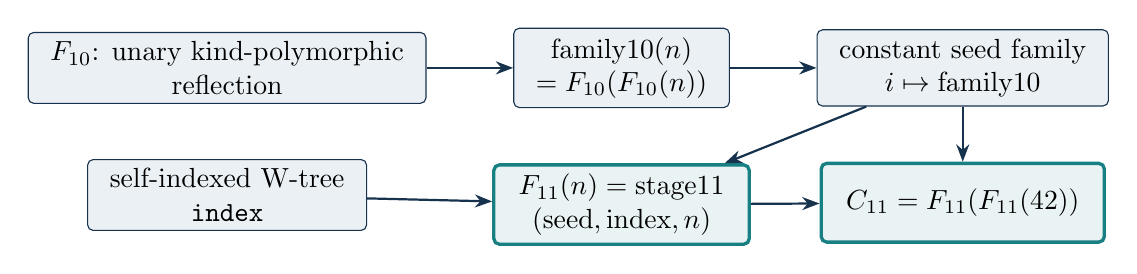
\begin{tikzpicture}[
  node distance=7mm and 11mm,
  box/.style={draw=navy,rounded corners=2pt,fill=bluegray,align=center,
    minimum height=9mm,inner xsep=8pt},
  strong/.style={draw=teal,very thick,rounded corners=2pt,fill=teal!9,
    align=center,minimum height=10mm,inner xsep=9pt},
  arr/.style={-{Stealth[length=2.2mm]},thick,draw=navy}
]
\node[box] (f10) {$F_{10}$: unary kind-polymorphic\\reflection};
\node[box,right=of f10] (fam) {$\mathrm{family10}(n)$\\$=F_{10}(F_{10}(n))$};
\node[box,right=of fam] (seed) {constant seed family\\$i\mapsto\mathrm{family10}$};
\node[box,below=of f10] (index) {self-indexed W-tree\\\lean{index}};
\node[strong,below=of fam] (stage) {$F_{11}(n)=\mathrm{stage11}$\\$(\mathrm{seed},\mathrm{index},n)$};
\node[strong,below=of seed] (c11) {$\Celeven=F_{11}(F_{11}(42))$};
\draw[arr] (f10)--(fam);
\draw[arr] (fam)--(seed);
\draw[arr] (index)--(stage);
\draw[arr] (seed)--(c11);
\draw[arr] (seed)--(stage);
\draw[arr] (stage)--(c11);
\end{tikzpicture}
\caption{The construction uses the predecessor's generating function as the
leaf seed and applies kind-polymorphic reflection at every node of the
self-indexed forest.}
\label{fig:architecture}
\end{figure}

%--------------------------------------------------------------------
\section{Formal domination theorems}

\subsection{One-step inequalities}

All basic estimates are consequences of membership in one of the two explicit
maxima.

\begin{lemma}[Visible oracle values]
If $i\le n$, then
\[
  fs(i,n)<R_{fs}(n).
\]
In Lean this is \lean{oracle\_lt\_reflect11}.
\end{lemma}

\begin{lemma}[Visible program values]
If $t\in\operatorname{Fk.ctmsUpTo}(n)$, then
\[
  \operatorname{Fk.fvalue}(\operatorname{packFamily}(fs),n,t)
  <R_{fs}(n).
\]
In Lean this is \lean{fvalue\_lt\_reflect11}.
\end{lemma}

\begin{lemma}[Input growth]
For every family $fs$ and input $n$, $n<R_{fs}(n)$.
\end{lemma}

These facts are independent of any monotonicity property of the evaluator.
They use only the finite maximum definitions and elementary arithmetic.

\subsection{Child-to-parent growth}

If $a=\operatorname{node}(g)$ and $i\le n$, then the $i$th child value appears
in the parent's prefix maximum:
\[
  \operatorname{stage}_{11}(\mathrm{seed},g(i),n)
  <\operatorname{stage}_{11}(\mathrm{seed},a,n).
\]
This is \lean{stage11\_child\_lt}.  It is the local edge relation used to embed
a chosen W-tree path into the global root hierarchy.

\subsection{Pointwise domination of the predecessor family}

\begin{theorem}[\lean{family10\_lt\_F11}]
For every $n\in\N$,
\[
   F_{10}(F_{10}(n))<F_{11}(n).
\]
\end{theorem}

\begin{proof}[Proof architecture]
The depth-zero term list contains the distinguished zero term, whose denoted
tree is proved by the existing theorem \lean{first\_tree\_leaf} to be a leaf.
There are therefore three explicit strict steps:
\[
\begin{aligned}
 \mathrm{family10}(n)
 &<\operatorname{stage}_{11}(\mathrm{seed},\mathrm{leaf},n)\\
 &<\operatorname{stage}_{11}(\mathrm{seed},\mathrm{treesOfDepth}(0),n)\\
 &<\operatorname{stage}_{11}(\mathrm{seed},\mathrm{index},n)=F_{11}(n).
\end{aligned}
\]
The first is inclusion of the seed at family index zero; the next two are
child-to-parent inequalities at index zero.  No evaluator monotonicity is used.
\end{proof}

\subsection{The required comparison}

\begin{theorem}[\lean{contender\_10\_lt\_contender\_11}]
\[
   \Cten<\Celeven.
\]
\end{theorem}

\begin{proof}
By definitional equality, $\Cten=\mathrm{family10}(42)$.  The pointwise theorem
gives
\[
  \Cten<F_{11}(42).
\]
Input growth, applied to the whole index tree at input $F_{11}(42)$, gives
\[
  F_{11}(42)<F_{11}(F_{11}(42))=\Celeven.
\]
Transitivity proves the claim.  This is exactly the Lean proof term.
\end{proof}

The certified margin is thus not ``old number plus one.''  The old number lies
below the \emph{inner} budget of the new diagonal, and the new hierarchy already
pointwise dominates the predecessor's full generating family.

\subsection{Program and tree domination}

Define the family visible at the root by
\[
  \operatorname{rootFamily11}(i,n)
   =\operatorname{stage}_{11}
      (\lambda\_.\mathrm{family10},\mathrm{treesOfDepth}(i),n).
\]
Then Lean proves:
\begin{theorem}[\lean{fvalue\_lt\_F11}]
For every $t\in\operatorname{Fk.ctmsUpTo}(n)$,
\[
 \operatorname{Fk.fvalue}
   (\operatorname{packFamily}(\operatorname{rootFamily11}),n,t)
 <F_{11}(n).
\]
\end{theorem}
At the final inner budget $n=F_{11}(42)$ this specializes to
\lean{fvalue\_lt\_contender\_11}: every enumerated kind-polymorphic program at
that budget is below $\Celeven$.

The index also remains cofinal for the W-language's denoted trees:
\begin{theorem}[\lean{defined\_tree\_eventually\_lt11}]
If $t$ occurs in the W-language enumeration at depth $k$, there is $N$ such
that for every $n\ge N$,
\[
  \operatorname{stage}_{11}(\mathrm{seed},\operatorname{defTree}(t),n)
  <F_{11}(n).
\]
\end{theorem}
The witness is explicit: if $t$ has list index $i$, take $N=k+i$ so both the
level $k$ and list position $i$ are visible in the corresponding prefix maxima.

%--------------------------------------------------------------------
\section{Why the number is computable in principle}

The value is physically infeasible to compute, but every component is total
and effective.

\begin{enumerate}[leftmargin=*]
\item \textbf{Finite syntax enumeration.}
  \lean{Fk.ctmsUpTo n} is a finite list generated by primitive recursion on
  $n$.  The list may be enormous, but it is computable.
\item \textbf{Decidable checking.}
  The Church-style kind-polymorphic checker uses a finite fuel parameter.  It
  may reject a valid term if fuel is insufficient, but accepted terms come with
  a sound typing derivation.
\item \textbf{Certified normalization.}
  \lean{Fk.sn\_of\_typed} supplies strong normalization for accepted erased
  terms with the oracle.  Well-founded recursion on that certificate computes a
  normal form, from which a Church numeral is decoded.
\item \textbf{Finite maxima.}
  \lean{prefixMax} and \lean{maximum} recurse over finite prefixes and lists.
\item \textbf{Structural W-recursion.}
  \lean{stage11} is a structurally accepted recursion on
  \lean{BigNumber.WTree Nat}; a node recursively exposes each proper child.
\item \textbf{Closed final term.}
  \lean{contender\_11} has type \lean{Nat} and no free variables, external
  functions, custom axioms, noncomputable definitions, unsafe code, or partial
  recursion.
\end{enumerate}

The proof objects underlying normalization may mention \lean{propext} and
\lean{Quot.sound}; these are precisely the axioms allowed by BusyLean.  They
occur in propositions and do not introduce a computational oracle into the
natural-number definition.

%--------------------------------------------------------------------
\section{Size analysis: formal facts and heuristic calibration}

\subsection{What is formally established}

The following chain is kernel-checked:
\[
  \Cten
  =\mathrm{family10}(42)
  <F_{11}(42)
  <F_{11}(F_{11}(42))
  =\Celeven.
\]
More generally,
\[
  \forall n\quad F_{10}(F_{10}(n))<F_{11}(n).
\]
At every node, $R_{fs}(n)$ simultaneously exceeds all visible child values and
all visible \Fk-program values relative to the packed child family.  Repeating
this node operation along \lean{index} is a genuine forest amplifier, not a
fixed finite stack written into the source.

\subsection{A deliberately cautious heuristic}

Let $\lvert\Fk\rvert$ informally denote the strength of the kind-polymorphic
normalizing language, and let $\iota$ denote the order type heuristically
represented by the W-language self-index.  A single reflection step acts like
adding one block of $\lvert\Fk\rvert$ above the oracle's growth rank; iteration
along a tree acts like transfinite repetition of that block.  The natural
informal description is therefore a hierarchy of the shape
\[
  f_{\lvert\Fk\rvert\cdot\iota}
\]
above a seed already containing two applications of $F_{10}$.  This notation is
only an explanatory metaphor.  No exact ordinal analysis of the repository's
kind-polymorphic system, its oracle extension, or the self-index has been
formalized, and this article does not assert one.

The robust conclusion does not depend on the heuristic: the pointwise family
comparison, program maximum, child inequalities, and final strict comparison
are formal Lean theorems.

\begin{center}
\begin{tabularx}{0.97\textwidth}{@{}>{\bfseries}lXX@{}}
\toprule
Feature & Contender 10 & Contender 11 \\
\midrule
Object language & kind-polymorphic $F_\omega$ & same certified language \\
Oracle interface & one unary oracle & encoded family of child-stage oracles \\
Amplifier & one reflection at each call to $F_{10}$ & reflection at every node of the self-indexed W-forest \\
Predecessor use & Contender 9 family as oracle & Contender 10 family as leaf seed \\
Uniform theorem & \lean{family9 n < F10 n} & \lean{family10 n < F11 n} \\
Program bound & programs at budget $F_{10}(42)$ & programs at budget $F_{11}(42)$ under the root family \\
Index theorem & none at this layer & every W-definable tree eventually dominated \\
Final number & $F_{10}(F_{10}(42))$ & $F_{11}(F_{11}(42))$ \\
\bottomrule
\end{tabularx}
\end{center}

%--------------------------------------------------------------------
\section{Verification and audit record}

\subsection{Remote kernel/elaborator check}

The verification run used Lean 4.34.0 and the exact BusyLean snapshot
\snapshot.  The 30 local modules in the transitive dependency closure of
\lean{BusyLean.Comparison10} were ordered topologically, concatenated after
removing only their import lines, and followed by the exact two source modules
in this archive.  The resulting unit was submitted to AXLE's \lean{check}
service with unbounded heartbeats and a 300 second request limit.

The recorded result was:
\begin{center}
\begin{tabular}{@{}ll@{}}
\toprule
Field & Result \\
\midrule
Lean environment & \lean{lean-4.34.0} \\
Compilation & \lean{okay = true} \\
Failed declarations & empty list \\
Lean errors & none \\
Combined check time & 8.900 seconds \\
Axioms of five principal new declarations & \lean{[propext, Quot.sound]} \\
Forbidden predecessor constants in $\Celeven$ closure & none \\
Transitive closure size reported by audit & 1,460 constants \\
\bottomrule
\end{tabular}
\end{center}

The five printed declarations were \lean{contender\_11}, the required comparison,
the pointwise family theorem, the W-tree eventual-domination theorem, and the
final program-bound theorem.  AXLE also returned an empty validation-failure
list, so no \lean{sorry}, unsafe declaration, or disallowed axiom was detected.

\subsection{What this check does and does not establish}

The merged verification is strong evidence because Lean parses, elaborates, and
kernel-checks the exact declarations against the exact dependency source.  It
also catches theorem holes, type errors, termination errors, and axiom-policy
violations.  It is not identical to a clean Lake build of the original module
graph: module import boundaries, generated object files, and the repository's
wall-clock budget harness are not exercised by a one-file merge.  Therefore the
archive includes \lean{scripts/check\_contender11.py}, which performs the official
staged build after integration:
\begin{enumerate}[leftmargin=*]
\item prebuild \lean{BusyLean.Comparison10} as accepted history;
\item time \lean{BusyLean.Contender11} against 15 seconds;
\item time \lean{BusyLean.Comparison11} against 60 seconds;
\item run \lean{test/Contender11Audit.lean}.
\end{enumerate}
Given that the entire merged current stack plus the new proof took under nine
seconds on the remote checker, the added modules are expected to fit comfortably,
but the supplied local script is the authoritative budget test.

%--------------------------------------------------------------------
\section{Engineering choices and rejected alternatives}

\subsection{Why explicit inclusion beats monotonicity}

It is tempting to claim that replacing an oracle by a larger oracle can only
increase a program's result.  That is false: a program can compare an oracle
answer with a numeral and take a smaller branch when the answer grows.  The
proof therefore identifies concrete entries in \lean{prefixMax} and
\lean{maximum}.  This method is robust under arbitrary oracle-sensitive
control flow and matches the repository's existing Contender 9 proof style.

\subsection{Why reuse the W-language index}

One might ask for an index generated by the kind-polymorphic language itself.
Its Church programs return natural numbers, not Lean W-trees, and the
normalization proof deliberately operates on erased syntax rather than a
set-theoretic model capable of returning infinitary trees.  The existing
W-language already supplies a certified universe of tree schedules and a
self-index theorem.  Reusing it isolates the new contribution to the stronger
reflection layer.

\subsection{Why not jump immediately to a kind-universe ladder}

The repository roadmap proposes stratified universes of kinds, allowing kinds
to quantify over lower-level kinds while placing the result one level higher.
That would be a genuine language-strength extension and may eventually dwarf
this proposal.  It also requires new syntax, kinding, substitution, conversion,
semantic domains, candidates, checker proofs, enumeration, and audit work.
Forest reflection over \lean{Fk} is already available conceptually and can be
proved with a small, reviewable delta.  Contender 11 is therefore a strong
conservative extension and a clean staging point before a universe-ladder
Contender 12.

\subsection{Why not use the incumbent constant}

Defining $\Celeven=G(\Cten)$ would make a numerical comparison easy but would
violate BusyLean's anti-laziness rule.  The present definition uses $F_{10}$ as
a reusable construction, forms the family $n\mapsto F_{10}(F_{10}(n))$, and
subjects that family to a qualitatively stronger forest reflection.  The
transitive dependency audit mechanically enforces this distinction.

%--------------------------------------------------------------------
\section{Further research questions}

\begin{enumerate}[leftmargin=*,label=\textbf{R\arabic*.}]
\item \textbf{Generic forest-reflection library.}
  Abstract the repeated Contender 9/11 pattern over a record containing a
  program enumeration, evaluator, unary-oracle packer, and domination lemmas.
  This could reduce future contenders to an instantiation plus a small proof.
\item \textbf{Kind-universe ladder.}
  Formalize levels $\Box_0\subset\Box_1\subset\cdots$ above the impredicative
  kind $\star$, prove normalization level by level, and diagonalize over the
  number of levels used by a program.
\item \textbf{Large elimination.}
  Add runtime-to-type dependency with certified large elimination, approaching
  a Calculus of Inductive Constructions style jump while retaining a total
  executable normalizer.
\item \textbf{Richer schedules.}
  Design a total language whose programs denote schedules for the
  kind-polymorphic reflection itself, rather than importing the older
  W-language index.  The central issue is a safe semantic interface from
  programs to well-founded trees.
\item \textbf{Formal ordinal lower bounds.}
  Define an internal fast-growing hierarchy and prove explicit embeddings of
  notation systems into \lean{stage11}.  Even a conservative lower bound would
  turn the current heuristic size discussion into a theorem.
\item \textbf{Checker completeness envelopes.}
  Quantify how much the fuel-bounded kind/type normalizer omits and prove that
  standard families of high-growth programs are accepted within explicit fuel
  bounds.
\item \textbf{Independent normalization audit.}
  Cross-check \lean{Fk.sn\_of\_typed} with a second logical relation or a
  translation into an independently formalized normalizing calculus.
\item \textbf{Build optimization.}
  Profile enumeration elaboration and generated code so that future language
  extensions remain comfortably inside the 15 second definition budget.
\item \textbf{No-\lean{Quot.sound} variant.}
  Investigate whether proof engineering can remove function extensionality
  dependencies from the new comparison layer, even if the inherited
  normalization development still uses them.
\item \textbf{Stronger diagonal policies.}
  Compare $F_{11}(F_{11}(42))$ with principled multi-parameter diagonals that
  separately grow the syntax budget, tree visibility bound, and child input,
  while avoiding arbitrary padding.
\end{enumerate}

%--------------------------------------------------------------------
\section{Reproducibility and archive layout}

The archive is organized for direct review and integration:
\begin{longtable}{@{}p{0.37\textwidth}p{0.57\textwidth}@{}}
\toprule
Path & Purpose \\
\midrule
\endhead
\lean{BusyLean/Contender11.lean} & Definitions of \lean{reflect11},
\lean{stage11}, \lean{family10}, \lean{rootFamily11}, \lean{F11}, and
\lean{contender\_11}. \\
\lean{BusyLean/Comparison11.lean} & One-step inequalities, pointwise family
comparison, required strict comparison, tree cofinality, and program bounds. \\
\lean{test/Contender11Audit.lean} & Axiom reports, predecessor-constant closure
audit, and declaration checks. \\
\lean{scripts/check\_contender11.py} & Staged clean build and official contest
budget check after integration. \\
\lean{scripts/verify\_axle.py} & Standard-library-only reproducer for the
pinned merged Lean 4.34.0 check. \\
\lean{patches/0001-contender11.patch} & Unified patch adding the modules and
updating the umbrella module, main audit, and timing configuration. \\
\lean{verification/AXLE\_REPORT.*} & Machine-readable and human-readable record
of the remote verification. \\
\lean{article/contender11.tex}, \lean{.pdf} & This research article and compiled
PDF. \\
\lean{MANIFEST.sha256} & SHA-256 digest of every packaged artifact. \\
\bottomrule
\end{longtable}

To integrate, copy the two Lean modules, append their imports to
\lean{BusyLean.lean}, copy the standalone audit and timing script, then run
\lean{python3 scripts/check\_contender11.py}.  At no point should any contender
be evaluated.

%--------------------------------------------------------------------
\section{Conclusion}

Contender 11 is a compact but genuine architectural advance over the current
BusyLean entry.  It preserves the strongest certified object language already
available---kind-polymorphic System $F_\omega$---and adds the repository's
strongest reusable amplifier: dynamically indexed family reflection iterated
along a self-indexed W-forest.  The result is closed and computable in principle,
uses only the allowed axioms, avoids every predecessor constant, pointwise
beats the predecessor's generating family, dominates all visible programs at
its final inner budget, and comes with a kernel-checked theorem
$\Cten<\Celeven$.

The design is intentionally conservative about unproved ordinal claims and
aggressive about formal auditability.  It is suitable for immediate integration
as Contender 11 and provides a clean base for the more ambitious kind-universe
and large-elimination programs suggested by the repository roadmap.

\begin{thebibliography}{9}

\bibitem{BusyLean}
BusyLean contributors.
\newblock \emph{BusyLean: name the biggest number, in Lean}.
\newblock Repository snapshot \snapshot, October 2026.

\bibitem{Girard1972}
Jean-Yves Girard.
\newblock \emph{Interpr\'etation fonctionnelle et \`elimination des coupures de
l'arithm\'etique d'ordre sup\'erieur}.
\newblock Th\`ese d'\'Etat, Universit\'e Paris VII, 1972.

\bibitem{Barendregt1992}
Henk P. Barendregt.
\newblock Lambda calculi with types.
\newblock In S. Abramsky, D. M. Gabbay, and T. S. E. Maibaum, editors,
\emph{Handbook of Logic in Computer Science}, volume 2, pages 117--309.
Oxford University Press, 1992.

\bibitem{Xin2026}
Jimmy Xin, Alex Schneidman, Chris Cummins, Karun Ram, Srihari Ganesh, and
Jannis Limperg.
\newblock AXLE: A cloud infrastructure for Lean 4 theorem proving utilities.
\newblock arXiv:2606.26442, 2026.

\end{thebibliography}

\appendix
\section{Complete Lean definition module}
\lstinputlisting{../BusyLean/Contender11.lean}

\section{Complete Lean comparison module}
\lstinputlisting{../BusyLean/Comparison11.lean}

\end{document}
